\documentclass[tikz]{standalone}

% === COMMANDS === (((
\newcommand{\head}[1]{
	\draw (#1) --++ (0,-1.5) --++ (-2,0) --++ (0,3) --++ (4,0) --++ (0,-4) 
	--++ (4.5,0);
}
\newcommand{\tail}[1]{
	\draw (#1) --++ (3.5,0) (#1)++(0,1) --++ (2.5,0) (#1)++(0,2) --++ (1.5,0);
}
\newcommand{\wing}[1]{
	\draw (#1) --++ (-3.5,0) (#1)++(0,-1) --++ (-2.5,0) (#1)++(0,-2) 
	--++ (-1.5,0) (#1)++(0,-3) --++ (-0.5,0) (#1)++(0.25,0.5) --++ (0,-4);
}
% )))

\begin{document}

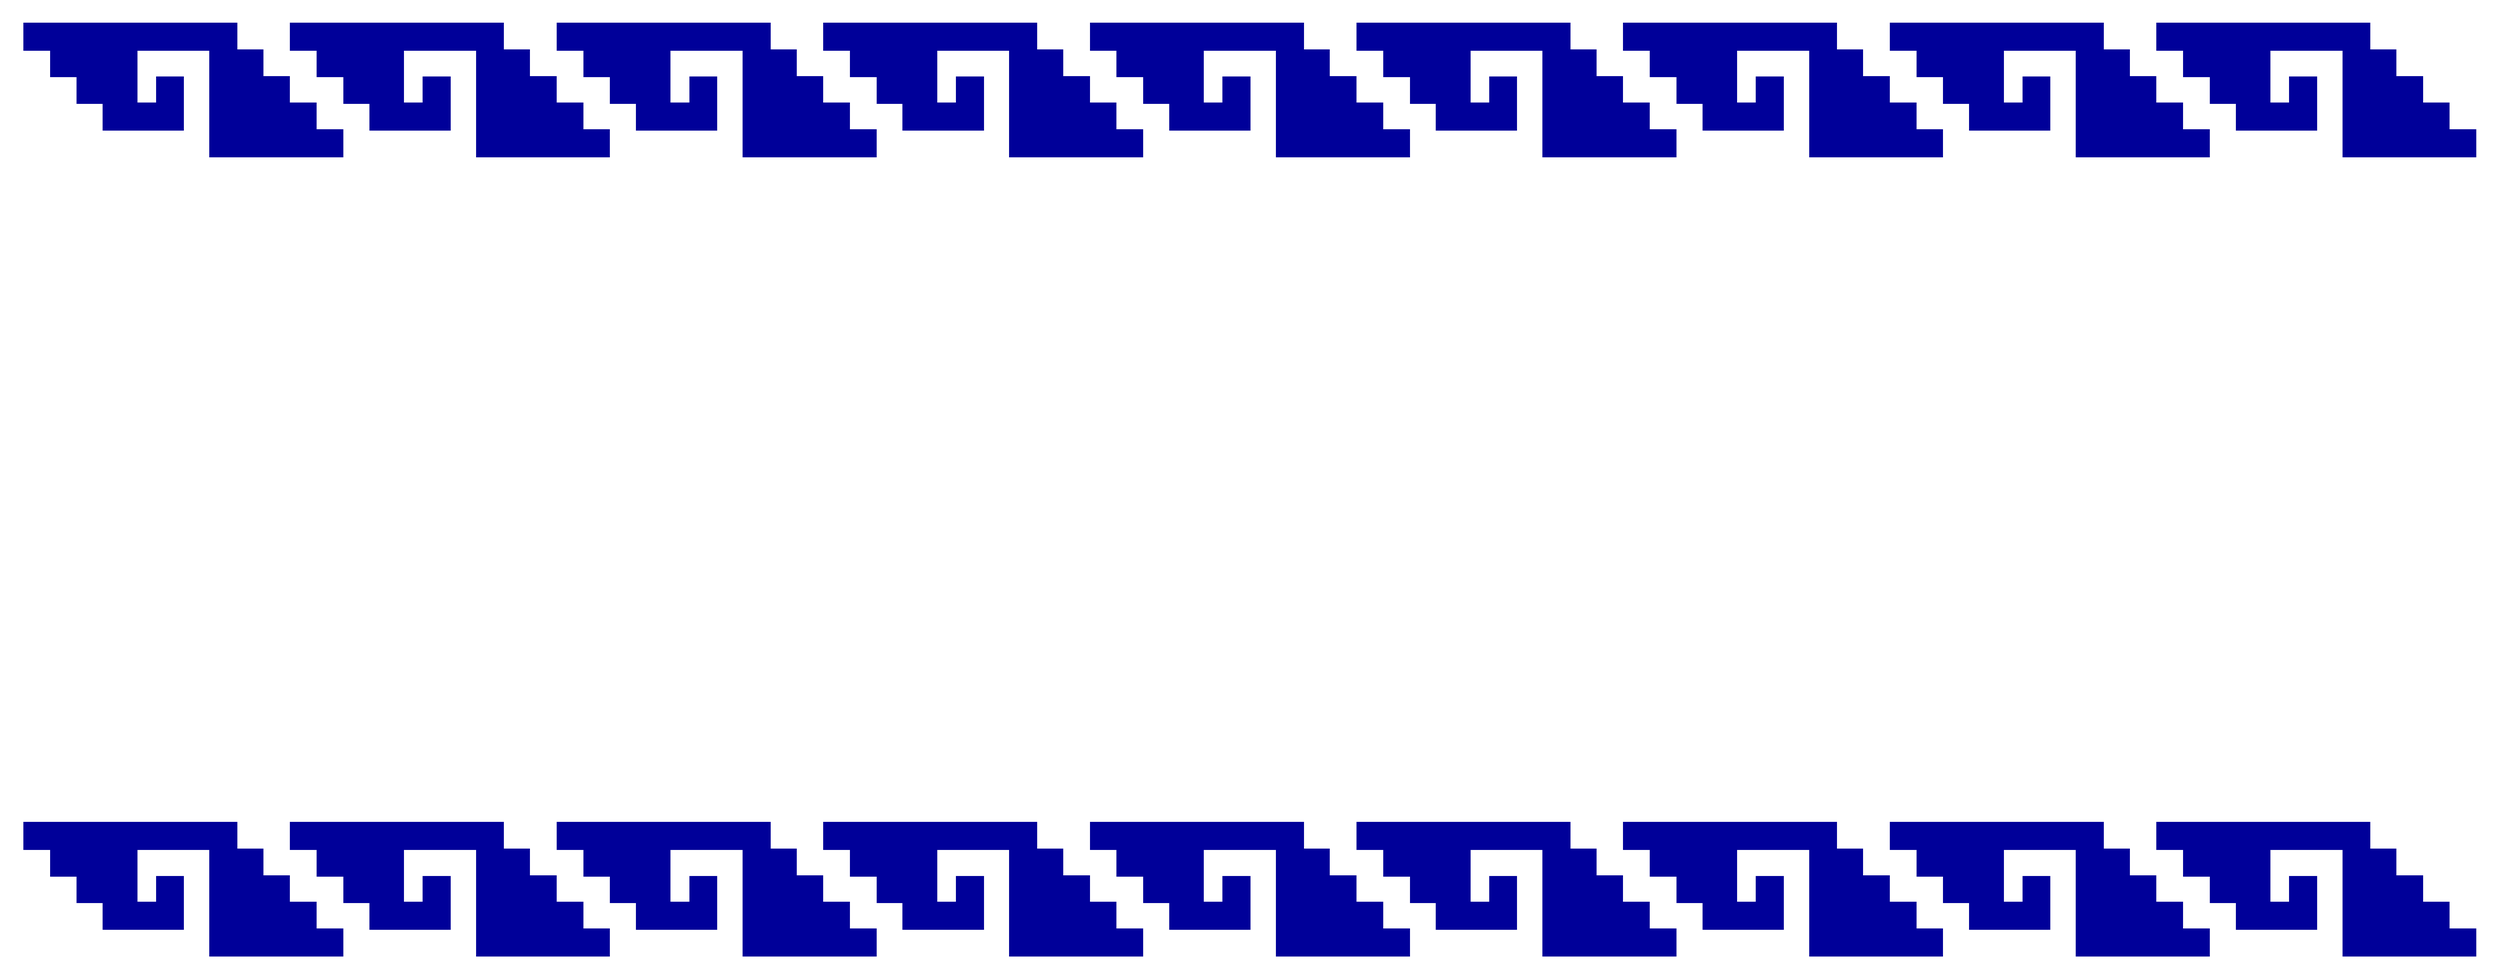
\begin{tikzpicture}
	[blue!60!black, line width=1.05cm]
	% \draw [help lines] (0,0) grid (30,5);
	\foreach \n in {0,...,8}{
		% up 
		\head{\n*10 + 2.5,3}
		\tail{\n*10 + 4.5,1.5}
		\wing{\n*10 + 0.5,4.5}
		% down 
		\head{\n*10 + 2.5,3-30}
		\tail{\n*10 + 4.5,1.5-30}
		\wing{\n*10 + 0.5,4.5-30}
	}
\end{tikzpicture}

\end{document}
